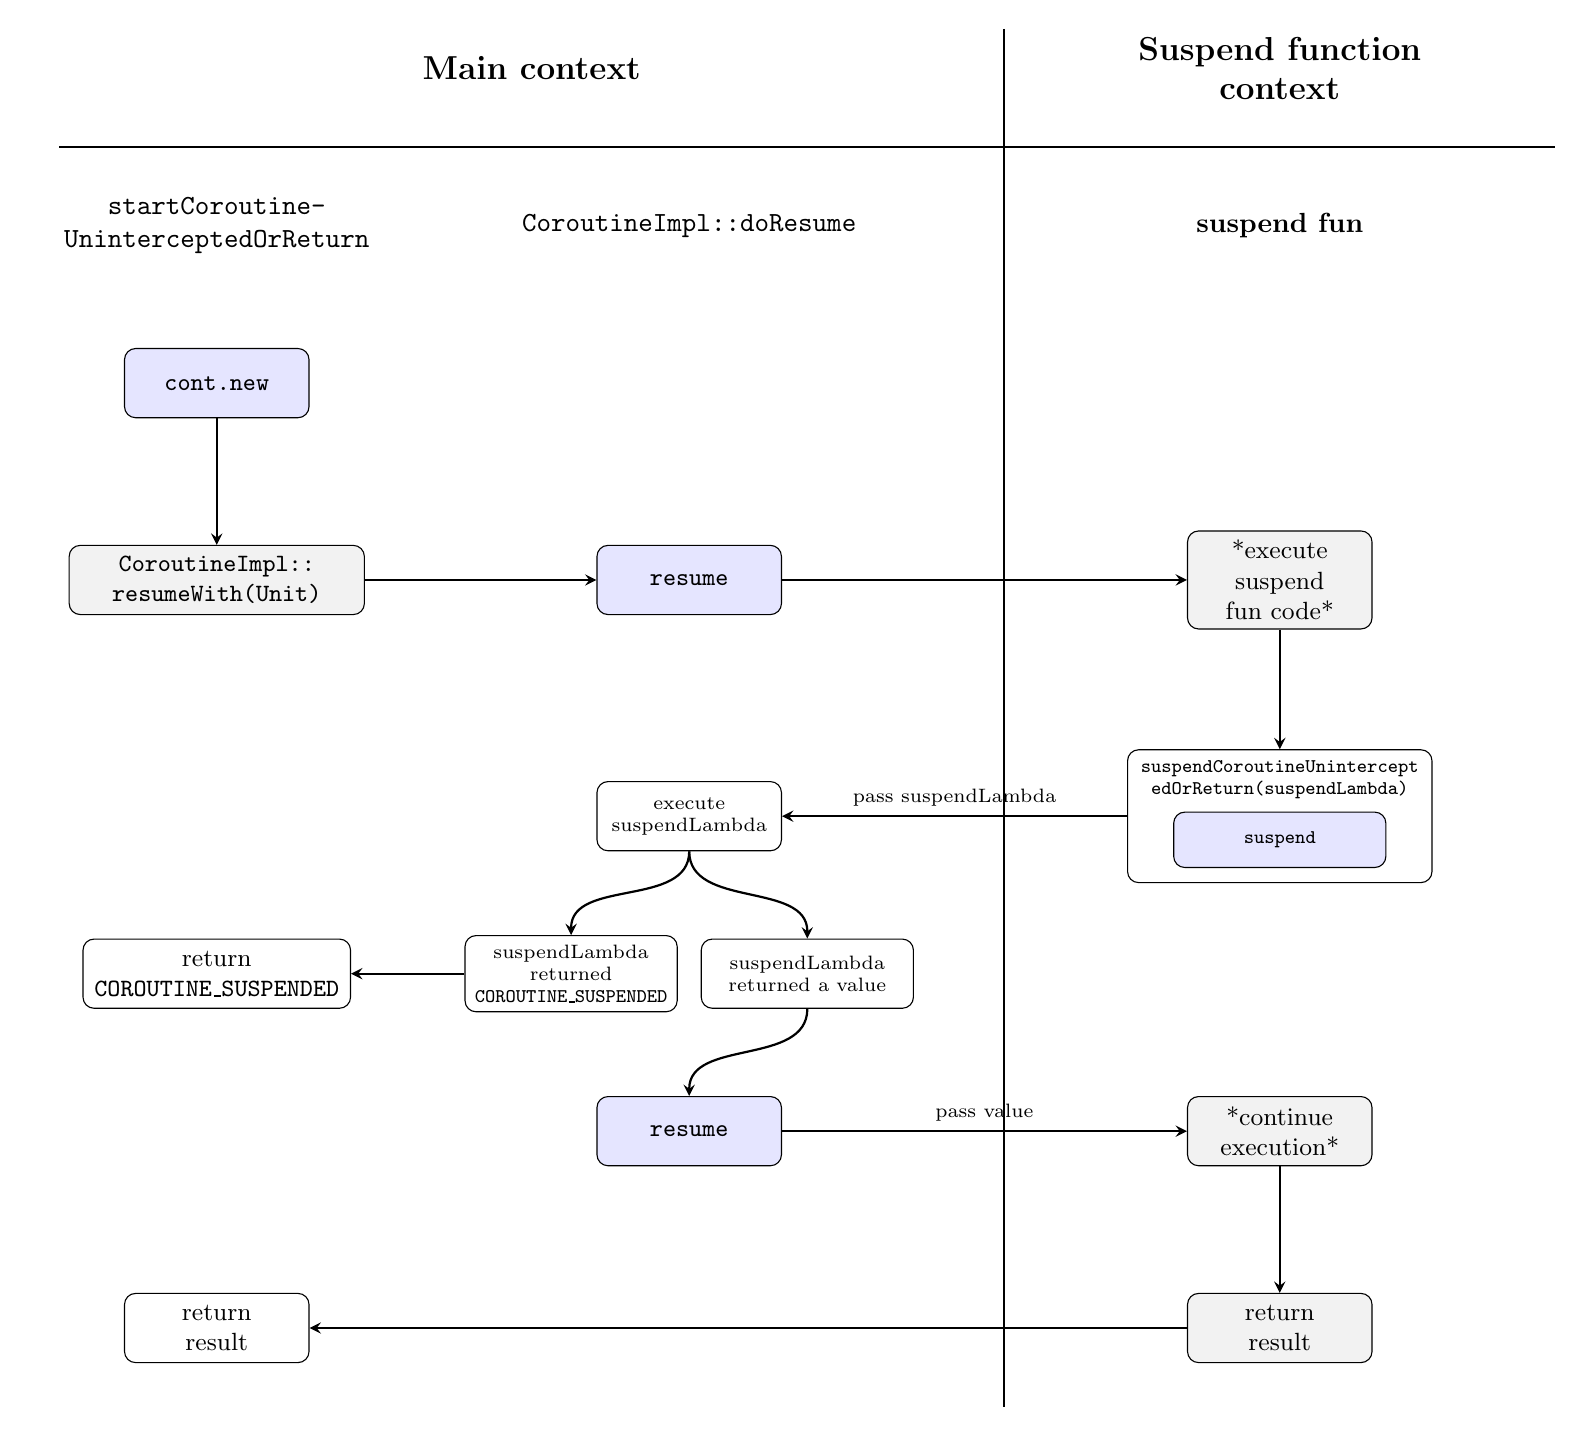
\begin{tikzpicture}[
    node distance=1.2cm and 3cm,
    every node/.style={font=\small},
    block/.style={rectangle, draw, fill=blue!10, text width=6em, text centered, rounded corners, minimum height=2.5em},
    decision/.style={diamond, draw, fill=yellow!10, text width=4em, text centered, aspect=2, inner sep=1pt},
    action/.style={rectangle, draw, fill=green!10, text width=7em, text centered, rounded corners, minimum height=2.5em},
    suspend/.style={rectangle, draw, fill=orange!20, text width=7em, text centered, rounded corners, minimum height=2.5em},
    title/.style={font=\large\bfseries, text width=13em, align=center},
    subtitle/.style={font=\normalsize\bfseries, text width=10em, align=center},
    whiteNote/.style={rectangle, draw, fill=white, text width=6em, text centered, rounded corners, minimum height=2.5em},
    blueNote/.style={rectangle, draw, fill=blue!10, text width=6em, text centered, rounded corners, minimum height=2.5em},
    yellowNote/.style={rectangle, draw, fill=gray!10, text width=6em, text centered, rounded corners, minimum height=2.5em},
    container/.style={rectangle, draw, fill=white!10, text width=8em, minimum height=6em, rounded corners},
    arrow/.style={->, >=stealth, thick},
    transfer/.style={->, >=stealth, thick},
    solidarrow/.style={->, >=stealth, thick},
    label/.style={font=\scriptsize, text=black}
]
% -------------------------
% Main Dividers
% -------------------------
    \draw[thick] (-2, 0) -- (17, 0); % Horizontal line
    \draw[thick] (10, 1.5) -- (10, -16); % Vertical line

% -------------------------
% Headers & Subheaders
% -------------------------
    \node[title] at (4, 1) {Main context};
    \node[title] at (13.5, 1) {Suspend function\\context};

    \node[subtitle, text width=13em] (sub1) at (0, -1) {\texttt{startCoroutine-\\UninterceptedOrReturn}};
    \node[subtitle, text width=13em] (sub2) at (6, -1) {\texttt{CoroutineImpl::doResume}};
    \node[subtitle, text width=10em] (sub3) at (13.5, -1) {suspend fun};

% -------------------------
% Nodes - Column 1 (X=0)
% -------------------------
    \node[blueNote] (n1_1) at (0, -3) {\texttt{cont.new}};
    \node[yellowNote, text width=10em] (n1_2) at (0, -5.5) {\texttt{CoroutineImpl::\\resumeWith(Unit)}};
    \node[whiteNote, text width=9em] (n1_3) at (0, -10.5) {return\\\texttt{COROUTINE\_SUSPENDED}};
    \node[whiteNote] (n1_4) at (0, -15) {return\\result};

% -------------------------
% Nodes - Column 2 (X=6) & Branches
% -------------------------
    \node[blueNote] (n2_1) at (6, -5.5) {\texttt{resume}};

    % Intermediate Branch Source (Centered under CoroutineImpl::doResume)
    \node[whiteNote, font=\scriptsize] (fork_src) at (6, -8.5) {execute\\suspendLambda};

    % Left Branch (X=4.5, centered around column)
    \node[whiteNote, font=\scriptsize, text width=7em] (fork_l) at (4.5, -10.5) {suspendLambda\\returned\\\texttt{COROUTINE\_SUSPENDED}};

    % Right Branch (X=7.5, centered around column)
    \node[whiteNote, font=\scriptsize, text width=7em] (fork_r) at (7.5, -10.5) {suspendLambda\\returned a value};

    \node[blueNote] (n2_2) at (6, -12.5) {\texttt{resume}};

% -------------------------
% Nodes - Column 3 (X=13.5)
% -------------------------
    \node[yellowNote] (n3_1) at (13.5, -5.5) {*execute\\suspend\\fun code*};

    % Container Box
    \node[container, minimum width=11em, minimum height=4.8em] (box) at (13.5, -8.5) {};
    \node[anchor=north, font=\scriptsize, text width=14em, align=center, inner sep=4pt] at (box.north) {\texttt{suspendCoroutineUnintercept\\edOrReturn(suspendLambda)}};
    \node[blueNote, font=\scriptsize, minimum height=2em, text width=7em] (n3_2) at (13.5, -8.8) {\texttt{suspend}};

    \node[yellowNote] (n3_3) at (13.5, -12.5) {*continue\\execution*};
    \node[yellowNote] (n3_4) at (13.5, -15) {return\\result};

% -------------------------
% Arrows & Routing
% -------------------------
    % Downward & Rightward Top Flow
    \draw[arrow] (n1_1) -- (n1_2);
    \draw[arrow] (n1_2) -- (n2_1);
    \draw[arrow] (n2_1) -- (n3_1);
    \draw[arrow] (n3_1) -- (box.north);

    % Arrow from container left side to execute suspendLambda
    \draw[arrow] (box.west) -- node[above, font=\scriptsize] {pass suspendLambda} (fork_src.east);

    % Fork Branching (Simulating the curly brace split)
    \draw[arrow] (fork_src.south) to[out=270, in=90] (fork_l.north);
    \draw[arrow] (fork_src.south) to[out=270, in=90] (fork_r.north);

    % Left Path Completion
    \draw[arrow] (fork_l) -- (n1_3);

    % Right Path Completion
    \draw[arrow] (fork_r) to[out=270, in=90] (n2_2);
    \draw[arrow] (n2_2) -- node[above, font=\scriptsize] {pass value} (n3_3);
    \draw[arrow] (n3_3) -- (n3_4);

    % Bottom Return (Updated to go directly across)
    \draw[arrow] (n3_4) -- (n1_4);
\end{tikzpicture}
